\begin{multicols}{2}
\section*{Objetivo General}
\normalsize{Determinar experimentalmente la aceleración gravitacional $g$ a partir de un experimento de caída libre.}\\
\section*{Objetivos específicos}
%\normalsize{
\begin{enumerate}
    \item Medir desplazamientos para un objeto en caída libre.
    \item Representar el movimiento del objeto mediante la construcción de gráficos que faciliten su análisis.
    \item Determinar la aceleración gravitacional $g$ experimentalmente.
\end{enumerate} 
%}\\
\section*{Referentes conceptuales}
El movimiento de un cuerpo en caída libre bajo la influencia de la gravedad es un ejemplo de aceleración constante. Esta aceleración, llamada aceleración gravitacional (g), tiene un valor aproximado de 9.77 m/s² en Bogotá, según un reporte de 1997, y está dirigida hacia el centro de la Tierra, ignorando factores como la rotación terrestre y la resistencia del aire.

\begin{center}
    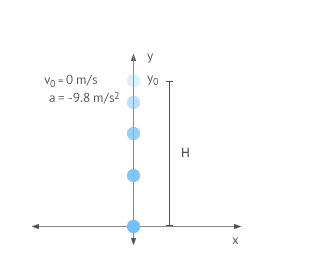
\includegraphics[scale=0.5]{fig/caida-libre.png}
\end{center}

La ecuación (\ref{eq1}) permite obtener la posición de un cuerpo en función del tiempo para una aceleración constante. Si el movimiento es completamente vertical su velocidad aumenta.

\begin{align}\label{eq1}
    y(t) = y_o + v_o \cdot t  - \dfrac{g t^2}{2}
\end{align}

Donde $y(t)$ representa la posición, $g$ la aceleración y $t$ el tiempo. Si el cuerpo “cae” desde el reposo $(v_o = 0)$ en un tiempo inicial $t_o = 0$. Si se define como $y_o = 0$ el punto desde donde se deja caer, por consiguiente, la ecuación anterior se reduce a:

\begin{align} \label{eq2}
    y(t) = - \dfrac{g t^2}{2}
\end{align}

\section*{Actividades Previas}   
\begin{enumerate}
\item Después de observar el vídeo de \parencite{valdes2024}, se concluye que g representa la aceleración debido a la gravedad en la superficie de la Tierra, mientras que G es la constante de gravitación universal, que describe la fuerza gravitatoria entre dos masas en cualquier lugar del universo, dependiendo directamente de las masas involucradas.

\item  En el punto más alto de una caída libre la velocidad siempre es 0 debido a que este es el punto donde se inicia el movimiento, y por ende no se le aplica una velocidad inicial, de lo contrario sería tiro vertical. 
        Sin embargo la aceleración es constante y su valor es de $-9.8 m/s^2$.
\item Diferencias y semejanzas que pueda tener un objeto en caída libre y un objeto lanzado de forma vertical hacia arriba:\\
    \textbf{Diferencias:}
    \begin{itemize}
        \item Un objeto en caída libre se mueve únicamente bajo la influencia de la gravedad, mientras que un objeto lanzado verticalmente hacia arriba tiene una velocidad inicial en contra de la gravedad.
    \end{itemize}

    \textbf{Semejanzas:}
    \begin{itemize}
        \item Los objetos en ambos movimientos tienen una aceleración constante en la dirección de la gravedad.
        \item Los objetos en ambos movimientos tienen una velocidad inicial o final de 0 (dependiendo si es caída libre o tiro vertical respectivamente) en el punto más alto de su trayectoria.
        \item Al alcanzar el punto más alto en un tiro vertical, el movimiento se transforma en caída libre.
    \end{itemize}
\item Tres personajes universales fueron importantes para hallar la aceleración gravitacional: \vspace{0.5cm} \\
    \textbf{Galileo Galilei:} Realizó experimentos con planos inclinados y péndulos, demostró que la aceleración de la gravedad es constante \parencite{serway2005fisica}.\\
    \textbf{Isaac Newton:} Propuso la ley de la gravitación universal, que describe la fuerza de atracción entre dos cuerpos \parencite{serway2005fisica}.\\
    \textbf{Henry Cavendish:} Utilizó una balanza de torsión para medir la constante de gravitación $G$. 
    La fuerza de atracción entre las esferas de plomo causaba una pequeña torsión en la barra suspendida \parencite{rsef2010}. 
    Un espejo en la barra reflejaba un rayo de luz, amplificando el ángulo de torsión. 
    Este ángulo era importante porque indicaba la magnitud de la torsión, que dependía de la fuerza entre las esferas. 
    Con esta medición, Cavendish calculó $G$ \parencite{fernando2017}.
\end{enumerate}

\begin{figure}[H]
    \caption{Proceso de Cavendish para medir la gravedad}
    \centering
    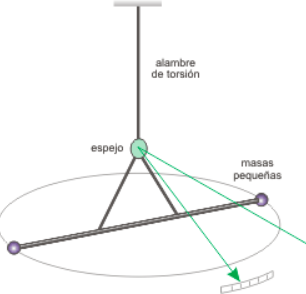
\includegraphics[scale=0.7]{fig/procesoCavendish-gravedad.png}
    \label{fig:procesoCavendish}
    \\Tomado de \parencite{ricuti2024}.
\end{figure}

\section*{Materiales de Laboratorio}  
\begin{itemize}
    \item Un celular con la aplicación PhyPhox establecida en el modo cronómetro acústico
    \item 30 globos
    \item Un flexómetro
    \item Una moneda de \$500
    \begin{center}
        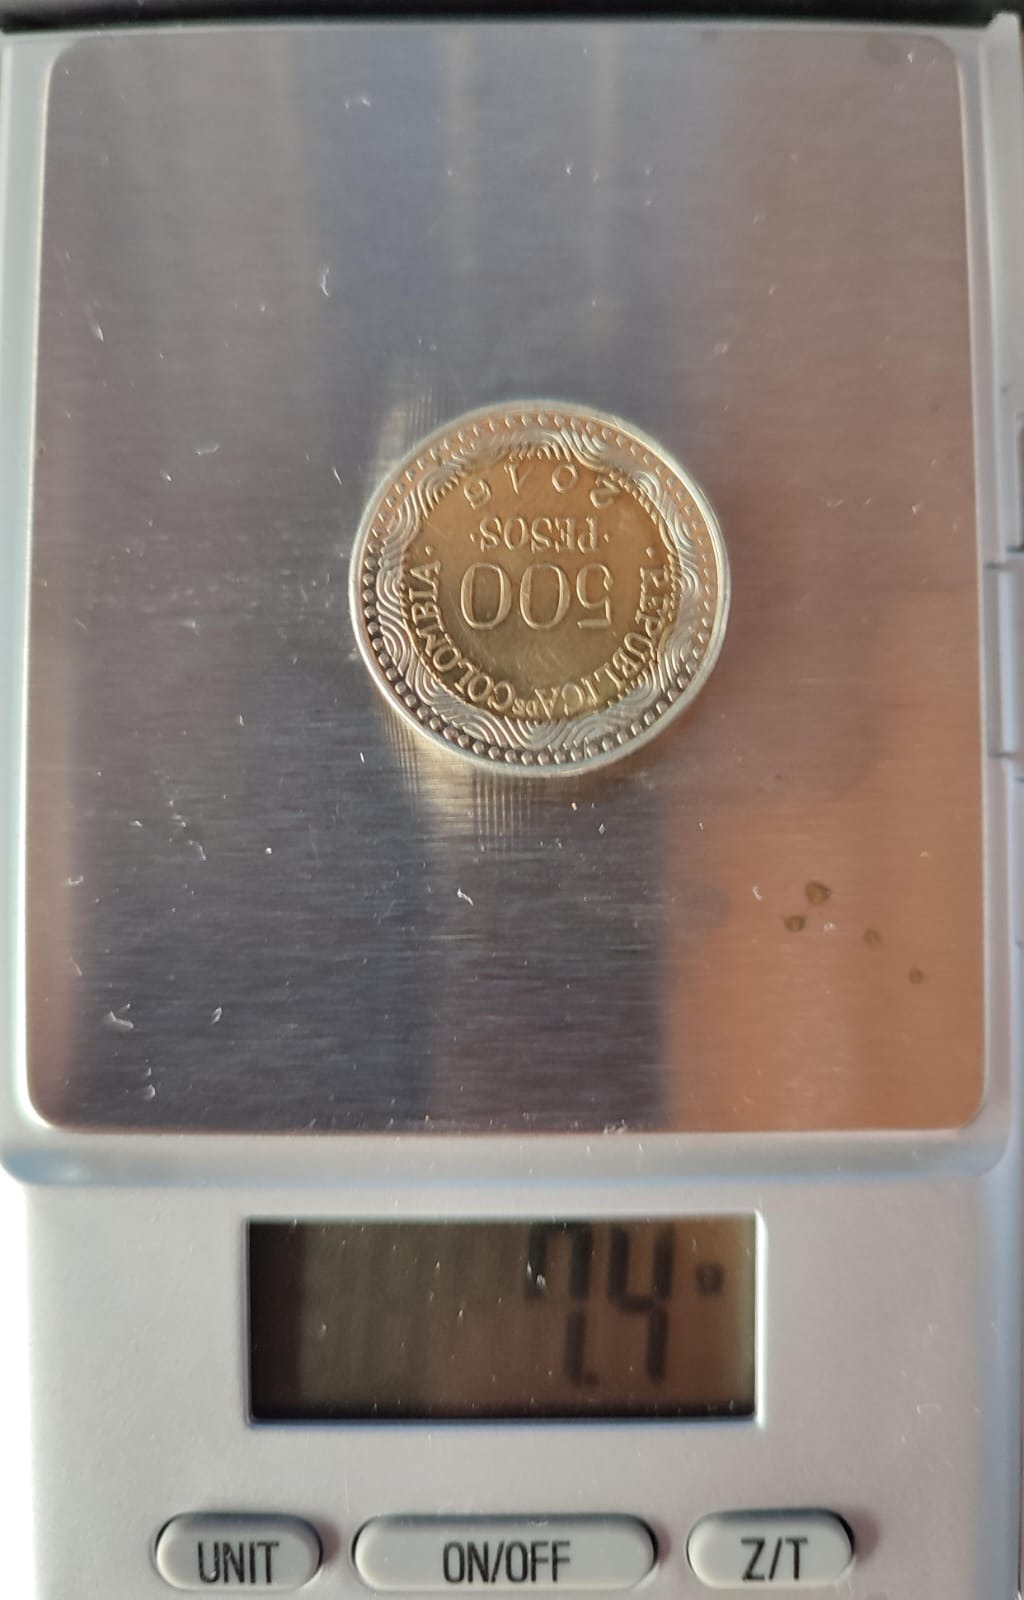
\includegraphics[scale=0.05]{fig/moneda.png}
    \end{center}
    \item Una pieza metálica
    \begin{center}
        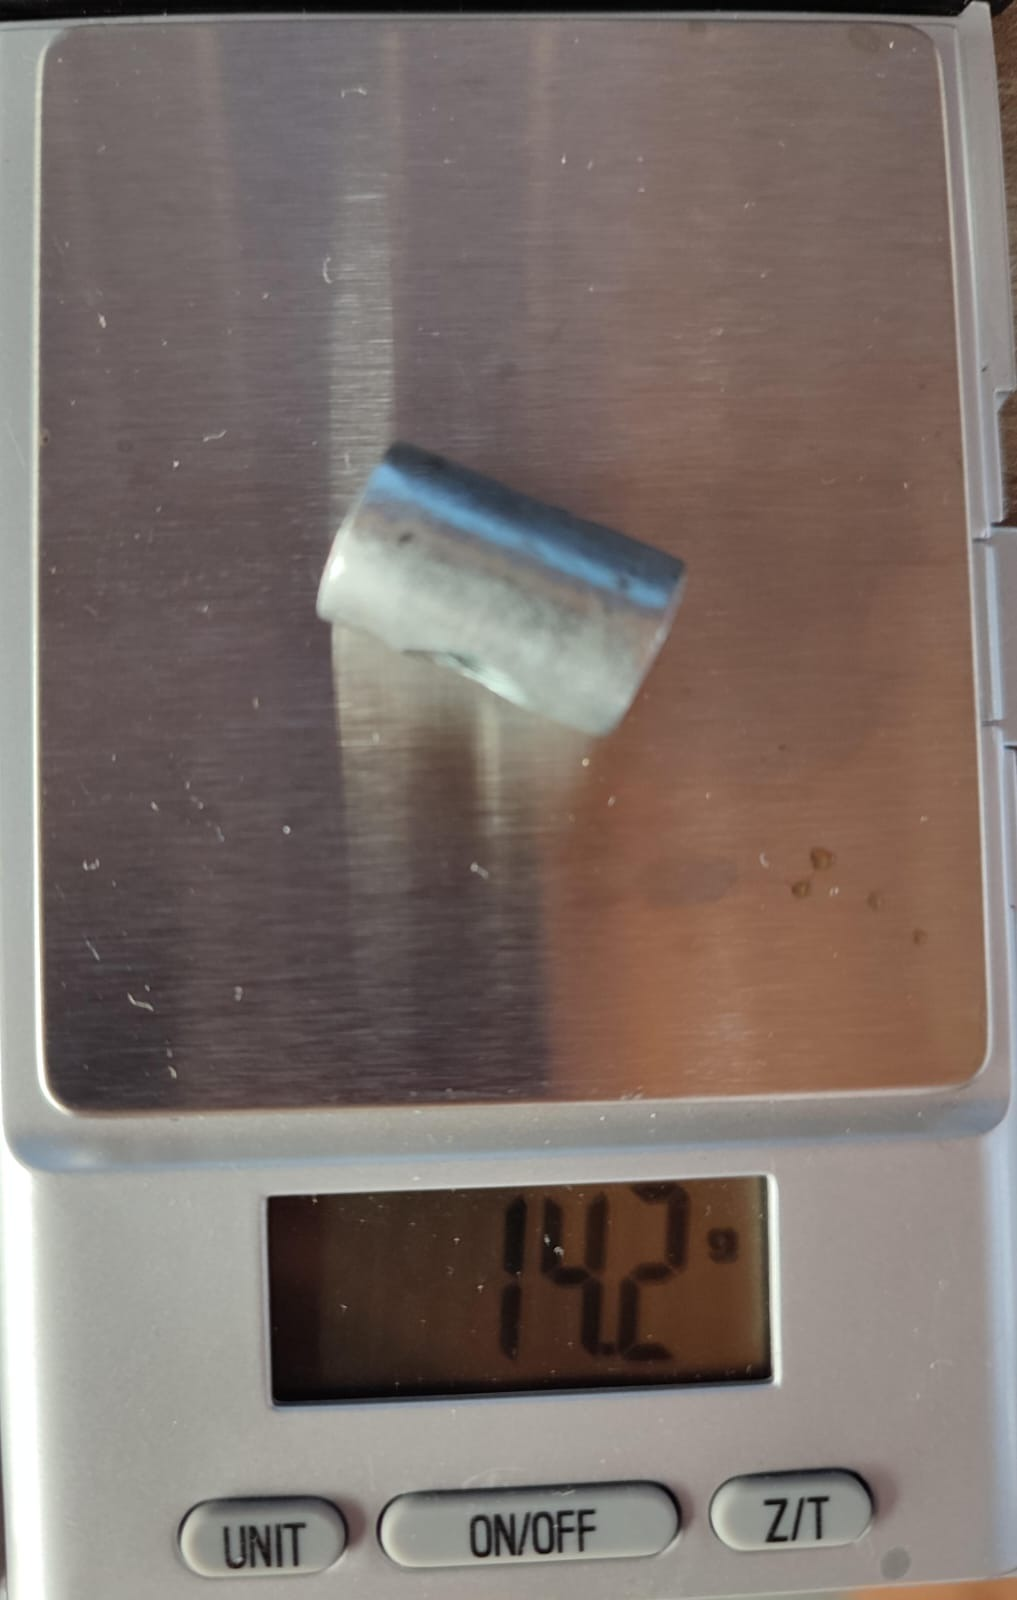
\includegraphics[scale=0.05]{fig/pieza-metalica.png}
    \end{center}
\end{itemize}

\section*{Procedimiento}
\begin{enumerate}
    \item Configurar la aplicación PhyPhox en el modo cronómetro acústico, ajustando el umbral a 0.2 y el retraso mínimo a 0.1.
    \item Colocar el móvil sobre una base estable en un área con suficiente altura y una superficie de impacto adecuada.
    \item Explotar el globo para iniciar la medición de tiempo y registrar tres mediciones para 5 alturas diferentes en la tabla 1.
    \item Repetir el experimento con un objeto de diferente peso y registrar los datos en la tabla 2.
\end{enumerate}

\begin{figure}[H]
    \caption{Montaje del experimento}
    \centering
    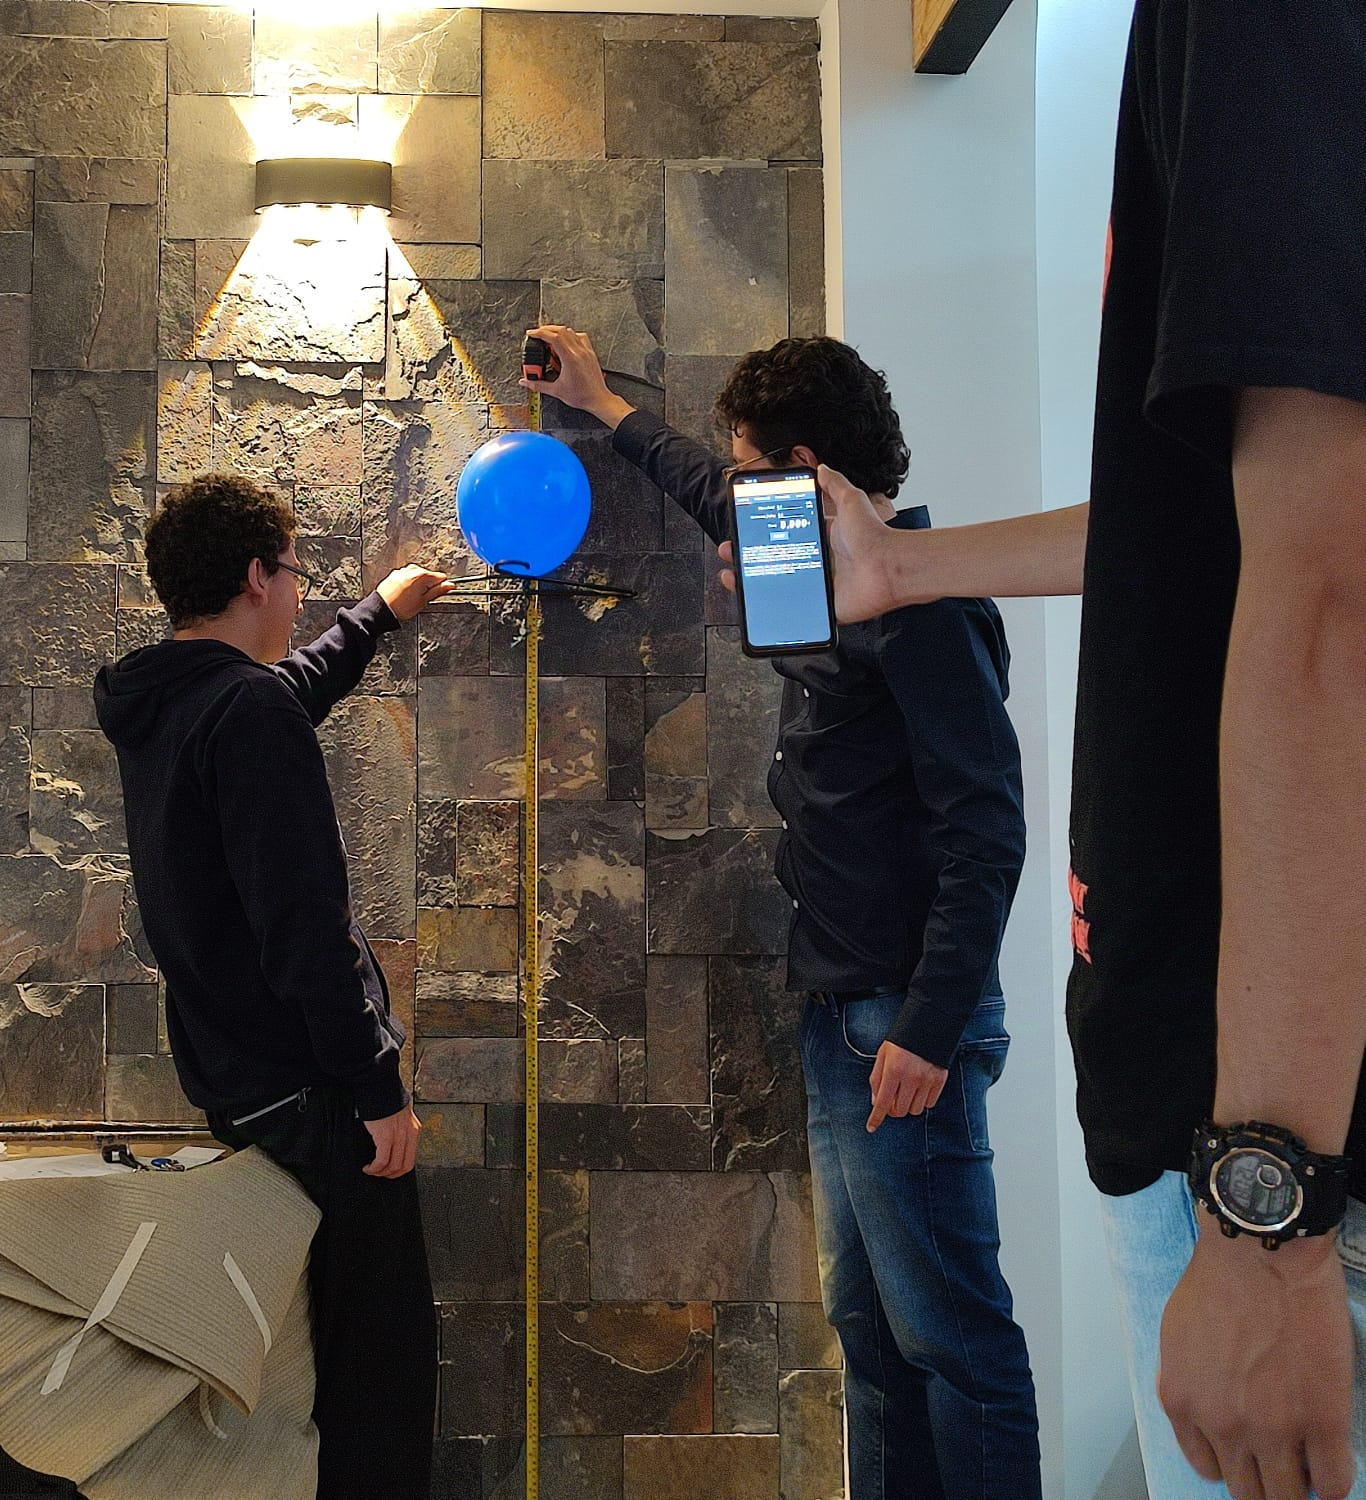
\includegraphics[scale=0.1]{fig/montaje.png}
    \label{fig:montaje}\\
    \textit{Nota: }Se observa cómo una persona sujeta el globo con el gancho, 
    otra persona registra el tiempo utilizando la aplicación PhyPhox, y una tercera mide la distancia.
\end{figure}



\section*{Resultados}
%Tabla 1
\begin{figure}[H]
    \caption{Datos de alturas y tiempos, objeto pesado}
    \centering
    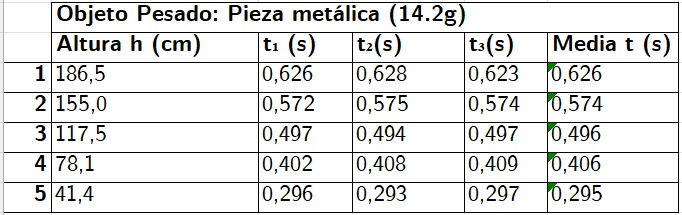
\includegraphics[scale=0.3]{fig/Tabla1-ObjetoPesado.png}
    \label{fig:tabla1}
\end{figure}

%Tabla 2
\begin{figure}[H]
    \caption{Datos de alturas y tiempos, objeto liviano}
    \centering
    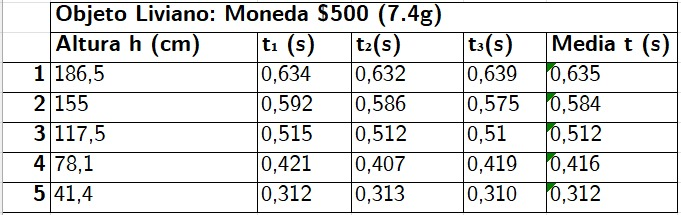
\includegraphics[scale=0.3]{fig/Tabla2-ObjetoLiviano.png}
    \label{fig:tabla2}
\end{figure}

\begin{figure}[H]
    \caption{Altura vs Tiempo, objeto Pesado}
    \centering
    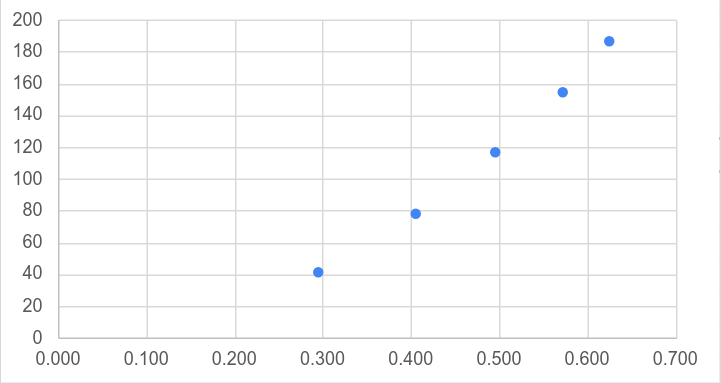
\includegraphics[scale=0.5]{fig/objPesado-Altura-Tiempo.png}
    \label{fig:h-t-obj-pesado}
\end{figure}

\vspace{-0.5cm}

\begin{figure}[H]
    \caption{Altura vs Tiempo, objeto Liviano}
    \centering
    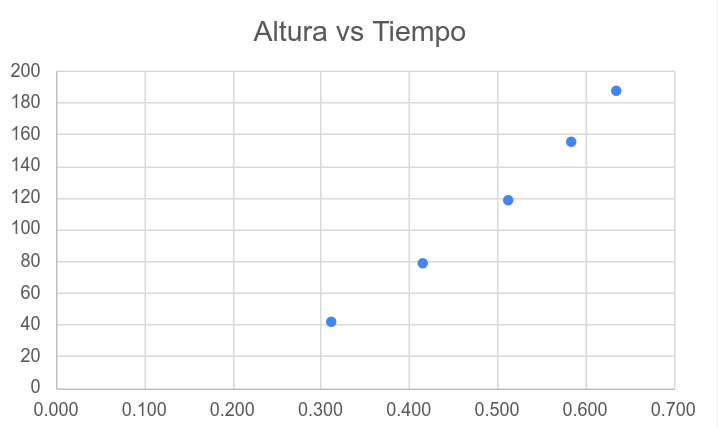
\includegraphics[scale=0.5]{fig/objLiviano-Altura-Tiempo.png}
    \label{fig:h-t-obj-liviano}
\end{figure}


Las figuras \ref{fig:h-t-obj-pesado} y \ref{fig:h-t-obj-liviano} muestran un comportamiento parabólico, esto es coherente con la teoría de caída libre, pues la gráfica de la ecuación (\ref{eq1}) del movimiento siempre es una parábola.
La altura aumenta rápidamente a medida que pasa el tiempo debido a que la gravedad acelera constantemente al objeto.

\textbf{Regresión por mínimos cuadrados}
%Tabla 3
\begin{figure}[H]
    \caption[scale=0.5]{Altura vs Tiempo Cuadrado}
    \centering
    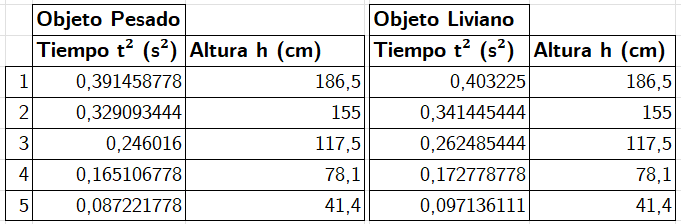
\includegraphics[scale=0.5]{fig/Tabla3-TiempoCuadrado.png}
\end{figure}

\textit{Nota: } Se decició hacer una regresión polinómica de grado 2 con los datos de las figuras (\ref{fig:tabla1}) y (\ref{fig:tabla2}), teniendo en cuenta los tiempos $t_1$, $t_2$ y $t_3$. De esta manera, se consiguue un valor de la gravedad más preciso.
\begin{figure}[H]
    \caption{Regresión para el objeto pesado}
    \centering
    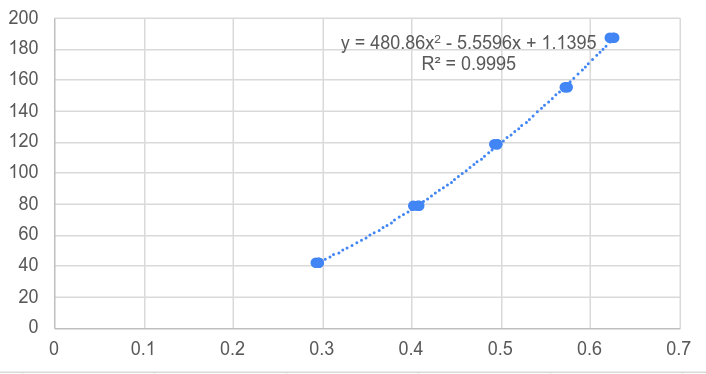
\includegraphics[scale=0.5]{fig/regresion-ObjetoPesado.png}
\end{figure}

\begin{figure}[H]
    \caption{Regresión para el objeto liviano}
    \centering
    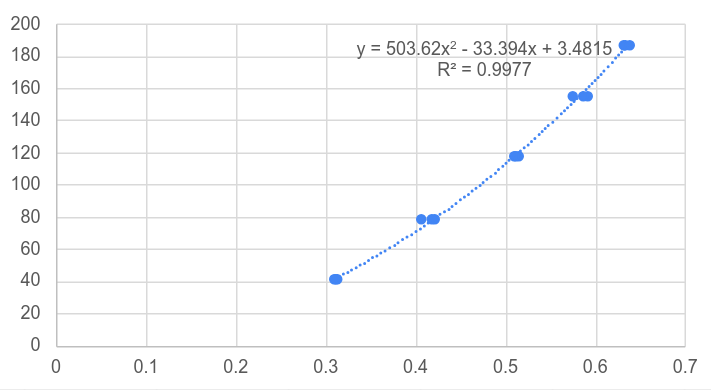
\includegraphics[scale=0.5]{fig/regresion-ObjetoLiviano.png}
\end{figure}

\textbf{Determinación de $g$} \\
Se obtuvieron las siguientes ecuaciones:

\begin{align}\label{eq3}
    y = 480.86x^2 - 5.5596x + 1.1395
\end{align}

\begin{align}\label{eq4}
    y = 503.62x^2 - 33.394x + 3.4815
\end{align}

Al usar la ecuación (\ref{eq2}) y compararla con (\ref{eq3}) y (\ref{eq4}), se obtiene que:
\begin{enumerate}
    \item $\dfrac{g}{2} = 480.86 \ cm/s^2$ \hspace{1cm} $g = 9.62 \ m/s^2$
    \item $\dfrac{g}{2} = 503.62 \ cm/s^2$ \hspace{1cm} $g = 10.07 \ m/s^2$
\end{enumerate}

\textbf{Calculo del error porcentual} \\

\[\text{Error\%} = \frac{|g_{\text{teórico}} - g_{\text{experimental}}|}{g_{\text{teórico}}} \times 100 \]

Para el objeto pesado: \[Error = \dfrac{|9.77 - 9.62|}{9.77} \times 100 = 1.53\%\] \\
Para el objeto liviano: \[Error = \dfrac{|9.77 - 10.07|}{9.77} \times 100 = 3.07\%\]

\begin{itemize}
    \item Con el objeto pesado se consigue un mejor valor de la gravedad, como se aprecia, el margen de error es bastante pequeño y el cáculo de los tiempos fue más sencillo.\\
    \item Con base en el montaje, las fuentes principales de error sistemático son: la precisión del cronómetro, el umbral y el retraso mínimo que se esbleció en PhyPhox, 
    la exactitud de la medida de la altura, el sonido ambiental y la posición en la que se dispuso el celular para escuchar los sonidos de inicio y fin del movimiento.\\
\end{itemize}


\section*{Conclusiones} 
\begin{itemize}
    \item Mediante las gráficas obtenidas se demostró que el movimiento de un objeto en caída libre sigue la forma de una parábola, además se comprobó que se trata de un movimiento variado, donde la aceleración es la gravedad.
    \item Se determinó experimentalmente el valor de la aceleración gravitacional $g$ con un error porcentual de 1.53\% y 3.07\% para el objeto pesado y liviano respectivamente.
    \item Se comprobó que con un objeto más pesado es más sencillo calcular el valor de la gravedad, debido a que a este objeto no le afecta tanto la resistencia con el aire.
    \item Para futuros laboratorios se recomienda realizar el mismo procedimiento con más alturas, de tal manera se podría obtener un valor más cercano a la gravedad en Bogotá.
\end{itemize}

\nocite{*} %incluyendo referencias que no se citaron, las que ya estaban
\printbibliography

\end{multicols}